\documentclass[10pt, a4paper, landscape]{article}

% ----- packages -----
\usepackage{amsmath} % AMS mathematical facilities for LaTeX
\usepackage{enumitem} % Control layout of itemize, enumerate, description
\usepackage{fancyhdr} % Extensive control of page headers and footers in LaTeX2
\usepackage{geometry} % Flexible and complete interface to document dimensions
\usepackage{graphicx} % Enhanced support for graphics
\usepackage{hyperref} % Extensive support for hypertext in LaTeX
\usepackage{multicol} % Intermix single and multiple columns
\usepackage{parskip} % Layout with zero \parindent, non-zero \parskip
\usepackage{tikz} % Create PostScript and PDF graphics in TeX
\usepackage{titlesec} % Select alternative section titles

% ----- tikz libraries -----
\usetikzlibrary{patterns}

% ----- random seed -----
\pgfmathsetseed{12}

% ----- custom commands -----
\newcommand{\E}{\mathrm{E}}
\newcommand{\Var}{\mathrm{Var}}
\newcommand{\se}{\mathrm{ee}}
\newcommand{\Cov}{\mathrm{Cov}}
\newcommand{\Corr}{\mathrm{Corr}}

% ----- page customization -----
\geometry{margin=1cm} % margins config
\pagenumbering{gobble} % remove page numeration
\setlength{\parskip}{0cm} % paragraph spacing
% title spacing
\titlespacing{\section}{0pt}{2ex}{1ex}
\titlespacing{\subsection}{0pt}{1ex}{0ex}
\titlespacing{\subsubsection}{0pt}{0.5ex}{0ex}

% ----- footer -----
\pagestyle{fancy}
\renewcommand{\headrulewidth}{0pt}
\cfoot{\href{https://github.com/marcelomijas/econometrics-cheatsheet}{\normalfont \footnotesize TS-24.12-ES - github.com/marcelomijas/econometrics-cheatsheet - CC-BY-4.0 license}}
\setlength{\footskip}{12pt}

% ----- document -----
\begin{document}
	\begin{multicols}{3}
		\begin{center}
			\textbf{\LARGE \href{https://github.com/marcelomijas/econometrics-cheatsheet}{Cheat Sheet Series de Tiempo}}
			
			{\footnotesize Por Marcelo Moreno - Universidad Rey Juan Carlos}
			
			{\footnotesize The Econometrics Cheat Sheet Project}
		\end{center}
		
		\section*{Conceptos básicos}
		
		\subsection*{Definiciones}
		
		\textbf{Serie temporal} - es una sucesión de observaciones cuantitativas de un fenómeno ordenadas en el tiempo.
		
		Hay algunas variaciones de serie temporal:
		
		\begin{itemize}[leftmargin=*]
			\item \textbf{Datos de panel} - consiste en una serie temporal para cada observación de una sección cruzada.
			\item \textbf{Secciones transversales agrupadas} - combina secciones cruzadas de diferentes periodos de tiempo.
		\end{itemize}
		
		\textbf{Proceso estocástico} - es una secuencia de variables aleatorias que están indexadas en el tiempo.
		
		\subsection*{Componentes de una serie temporal}
		
		\begin{itemize}[leftmargin=*]
			\item \textbf{Tendencia} - es el movimiento general a l/p de una serie.
			\item \textbf{Variaciones estacionales} - son oscilaciones periódicas que son producidas en un período igual o inferior al año, y pueden ser fácilmente identificadas en diferentes años (usualmente son el resultado de la climatología).
			\item \textbf{Ciclo} - son oscilaciones periódicas que se producen en un periodo mayor al año (son resultado del ciclo económico).
			\item \textbf{Variaciones residuales} - son movimientos que no siguen una oscilación periódica identificable (resultado de fenómenos eventuales no permanentes que pueden afectar a la variable estudiada en un momento dado).
		\end{itemize}
		
		\subsection*{Tipos de modelos de series temporales}
		
		\begin{itemize}[leftmargin=*]
			\item \textbf{Modelos estáticos} - la relación entre $y$ y $x$'s es contemporánea. Conceptualmente:
			
			\begin{center}
				$y_{t} = \beta_{0} + \beta_{1} x_{t} + u_{t}$
			\end{center}
			
			\item \textbf{Modelos de rezagos distribuidos} - la relación entre $y$ y $x$'s no es contemporánea. Conceptualmente:
			
			\begin{center}
				$y_{t} = \beta_{0} + \beta_{1} x_{t} + \beta_{2} x_{t - 1} + \cdots + \beta_{s} x_{t - (s - 1)} + u_{t}$
			\end{center}
			
			El efecto acumulado a largo plazo en $y$ cuando $\Delta x$ es:
			
			\begin{center}
				$\beta_{1} + \beta_{2} + \cdots + \beta_{s}$
			\end{center}
			
			\item \textbf{Modelos dinámicos} - un rezago de la variable dependiente es parte de las variables independientes (endogeneidad). Conceptualmente:
			
			\begin{center}
				$y_{t} = \beta_{0} + \beta_{1} y_{t - 1} + \cdots + \beta_{s} y_{t - s} + u_{t}$
			\end{center}
			
			\item Combinaciones de lo anterior, como modelos de rezagos distribuidos racionales (rezagos distribuidos + dinámicos).
		\end{itemize}
		
		\columnbreak
		
		\section*{Supuestos y propiedades}
		
		\subsection*{Supuestos MCO bajo series temporales}
		
		Bajo estos supuestos, los estimadores de los parámetros MCO presentarán buenas propiedades. \textbf{Supuestos Gauss-Markov} extendidos en series temporales:
		
		\begin{enumerate}[leftmargin=*, label=t\arabic{*}.]
			\item \textbf{Linealidad de parámetros y dependencia débil}.
			
			\begin{enumerate}[leftmargin=*, label=\alph{*}.]
				\item $y_{t}$ debe ser una función lineal de $\beta$'s.
				\item El proceso estocástico $\lbrace( x_{t}, y_{t}) : t = 1, 2, \ldots, T \rbrace$ es estacionario y débilmente dependiente.
			\end{enumerate}
			
			\item \textbf{No colinealidad perfecta}.
			
			\begin{itemize}[leftmargin=*]
				\item No hay variables independientes que sean constantes: $\Var(x_{j}) \neq 0, \; \forall j = 1, \ldots, k$
				\item No hay una relación lineal exacta entre variables independientes.
			\end{itemize}
			
			\item \textbf{Media condicional cero y correlación cero}.
			
			\begin{enumerate}[leftmargin=*, label=\alph{*}.]
				\item No hay errores sistemáticos: $\E(u \mid x_{1}, \ldots, x_{k}) = \E(u) = 0 \rightarrow$ \textbf{exogeneidad fuerte} (a implica b).
				\item No hay variables relevantes no incluidas en el modelo: $\Cov(x_{j} , u) = 0, \; \forall j = 1, \ldots, k \rightarrow$ \textbf{exogeneidad débil}.
			\end{enumerate}
			
			\item \textbf{Homocedasticidad}. La variabilidad de los resid. es igual para cualquier nivel de $x$: $\Var(u \mid x_{1}, \ldots, x_{k}) = \sigma^{2}_{u}$
			\item \textbf{No autocorrelación}. Los residuos no contienen información sobre otros residuos: \\
			$\Corr(u_{t}, u_{s} \mid x_{1}, \ldots, x_{k}) = 0, \; \forall t \neq s$
			\item \textbf{Normalidad}. Los residuos son independientes e idénticamente distribuidos (\textbf{i.i.d.}): $u \sim \mathcal{N}(0, \sigma^{2}_{u})$
			\item \textbf{Tamaño de datos}. El número de observaciones disponibles debe ser mayor a $(k + 1)$ parámetros a estimar. (Ya satisfecho bajo situaciones asintóticas)
		\end{enumerate}
		
		\subsection*{Propiedades asintóticas de MCO}
		
		Bajo los supuestos del modelo econométrico y el Teorema Central del Límite:
		
		\begin{itemize}[leftmargin=*]
			\item De t1 a t3a: MCO es \textbf{insesgado}. $\E(\hat{\beta}_{j}) = \beta_{j}$
			\item De t1 a t3: MCO es \textbf{consistente}. $\mathrm{plim}(\hat{\beta}_{j}) = \beta_{j}$ (a t3b sin t3a, exogeneidad débil, insesg. y consistente).
			\item De t1 a t5: \textbf{normalidad asintótica} de MCO (entonces, t6 es necesariamente satisfecho): $u \underset{a}{\sim}\mathcal{N}(0, \sigma^{2}_{u})$
			\item De t1 a t5: \textbf{estimador insesgado} de $\sigma^{2}_{u}$. $\E(\hat{\sigma}^{2}_{u}) = \sigma^{2}_{u}$
			\item De t1 a t5: MCO es MELI (Mejor Estimador Lineal Insesgado, \textcolor{blue}{BLUE} en inglés) or \textbf{eficiente}.
			\item De t1 a t6: contrastes de hipótesis e intervalos de confianza son fiables.
		\end{itemize}
		
		\columnbreak
		
		\section*{Tendencia y estacionalidad}
		
		\textbf{Regresión espuria} - es cuando la relación entre $y$ y $x$ es debida a factores que afectan a $y$ y que tienen correlación con $x$, $\Corr(x_{j}, u) \neq 0$. Es el \textbf{incumplimiento de t3}.
		
		\subsection*{Tendencia}
		
		Dos series temporales pueden tener la misma (o contraria) tendencia, lo que lleva a altos niveles de correlación. Esto provoca una falsa apariencia de causalidad, el problema es \textbf{regresión espuria}. Dado el modelo:
		
		\begin{center}
			$y_{t} = \beta_{0} + \beta_{1} x_{t} + u_{t}$
		\end{center}
		
		donde:
		
		\begin{center}
			$y_{t} = \alpha_{0} + \alpha_{1} \mathrm{Tendencia}+ v_{t}$
			
			$x_{t} = \gamma_{0} + \gamma_{1} \mathrm{Tendencia}+ v_{t}$
		\end{center}
		
		Añadir una tendencia al modelo puede resolver el problema:
		
		\begin{center}
			$y_{t} = \beta_{0} + \beta_{1} x_{t} + \beta_{2} \mathrm{Tendencia}+ u_{t}$
		\end{center}
		
		Una tendencia puede ser lineal o no lineal (cuadrática, cúbica, exponencial, etc.)
		
		Otra manera, es hacer uso del \textbf{filtro Hodrick-Prescott} y extraer la tendencia y el componente cíclico.
		
		\subsection*{Estacionalidad}
		
		\setlength{\multicolsep}{0pt}
		\begin{multicols}{2}
			Una serie temporal puede manifestar estacionalidad. Esto es, que la serie está sujeta a variaciones estacionales o patrones usualmente relacionados al clima.
			
			Por ejemplo, el PIB (negro) es usualmente mayor en verano y menor en invierno. Serie ajustada estacionalmente ({\color{red} rojo}) en comparación.
			
			\columnbreak
			
			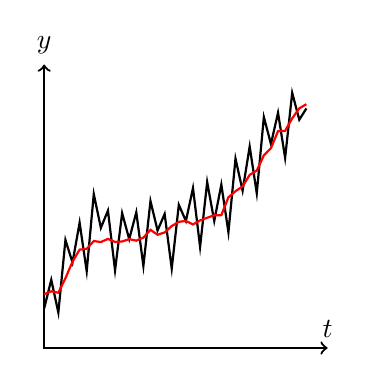
\begin{tikzpicture}[scale=0.18]
				% \draw [step=1, gray, very thin] (0, 0) grid (20, 20);
				\draw [thick, <->] (0, 20) node [anchor=south] {$y$} -- (0, 0) -- (20, 0) node [anchor=south] {$t$};
				\draw [thick, black] 
				(0.0, 2.794) -- (0.5, 4.810) -- 
				(1.0, 2.500) -- (1.5, 7.619) -- 
				(2.0, 6.031) -- (2.5, 8.840) -- 
				(3.0, 5.420) -- (3.5, 10.855) -- 
				(4.0, 8.474) -- (4.5, 9.695) -- 
				(5.0, 5.481) -- (5.5, 9.512) -- 
				(6.0, 7.680) -- (6.5, 9.573) -- 
				(7.0, 5.787) -- (7.5, 10.366) -- 
				(8.0, 8.291) -- (8.5, 9.451) -- 
				(9.0, 5.604) -- (9.5, 10.099) -- 
				(10.0, 8.962) -- (10.5, 11.282) -- 
				(11.0, 7.130) -- (11.5, 11.709) -- 
				(12.0, 8.962) -- (12.5, 11.526) -- 
				(13.0, 8.168) -- (13.5, 13.358) -- 
				(14.0, 11.099) -- (14.5, 14.213) -- 
				(15.0, 10.916) -- (15.5, 16.290) -- 
				(16.0, 14.396) -- (16.5, 16.595) -- 
				(17.0, 13.419) -- (17.5, 18.000) -- 
				(18.0, 16.106) -- (18.5, 16.900); 
				\draw [thick, red] 
				(0.0, 3.7939) -- (0.5, 3.9982) -- 
				(1.0, 3.9000) -- (1.5, 4.9183) -- 
				(2.0, 6.0905) -- (2.5, 6.9397) -- 
				(3.0, 6.9998) -- (3.5, 7.5450) -- 
				(4.0, 7.4733) -- (4.5, 7.6947) -- 
				(5.0, 7.4809) -- (5.5, 7.5115) -- 
				(6.0, 7.6794) -- (6.5, 7.5725) -- 
				(7.0, 7.7863) -- (7.5, 8.3336) -- 
				(8.0, 7.9901) -- (8.5, 8.1504) -- 
				(9.0, 8.6031) -- (9.5, 8.9008) -- 
				(10.0, 8.9618) -- (10.5, 8.7176) -- 
				(11.0, 8.9998) -- (11.5, 9.1901) -- 
				(12.0, 9.3618) -- (12.5, 9.3733) -- 
				(13.0, 10.6321) -- (13.5, 11.0588) --
				(14.0, 11.3992) -- (14.5, 12.2137) -- 
				(15.0, 12.5160) -- (15.5, 13.5901) -- 
				(16.0, 14.0969) -- (16.5, 15.2954) -- 
				(17.0, 15.3198) -- (17.5, 16.2000) -- 
				(18.0, 16.9069) -- (18.5, 17.2008);
			\end{tikzpicture}
		\end{multicols}
		
		\begin{itemize}[leftmargin=*]
			\item Este problema es \textbf{regresión espuria}. Un ajuste estacional puede solucionarlo.
		\end{itemize}
		
		Un \textbf{ajuste estacional} sencillo es crear variables estacionales binarias y añadirlas al modelo. Por ejemplo, una serie trimestral ($Qq_{t}$ son variables binarias):
		
		\begin{center}
			$y_{t} = \beta_{0} + \beta_{1} Q2_{t} + \beta_{2} Q3_{t} + \beta_{3} Q4_{t} + \beta_{4} x_{1t} + \cdots + \beta_{k} x_{kt} + u_{t}$
		\end{center}
		
		Otro método es ajustar estacionalmente (sa) las variables, y entonces, hacer la regresión con las variables ajustadas:
		
		\begin{center}
			$z_{t} = \beta_{0} + \beta_{1} Q2_{t} + \beta_{2} Q3_{t} + \beta_{3} Q4_{t} + v_{t} \rightarrow \hat{v}_{t} + \E(z_{t}) = \hat{z}_{t}^{sa}$
			
			$\hat{y}_{t}^{sa}= \beta_{0} + \beta_{1} \hat{x}_{1t}^{sa} + \cdots + \beta_{k} \hat{x}_{kt}^{sa} + u_{t}$
		\end{center}
		
		Hay métodos mucho mejores y complejos para ajustar estacionalmente, como el \textbf{X-13ARIMA-SEATS}.
		
		\columnbreak
		
		\section*{Autocorrelación}
		
		El residuo de cualquier observación, $u_{t}$, está correlacionado con el residuo de cualquier otra observación. Las observaciones no son independientes. Es el \textbf{incumplimiento} de \textbf{t5}.
		
		\begin{center}
			$\Corr(u_{t}, u_{s} \mid x_{1}, \ldots, x_{k}) = \Corr(u_{t}, u_{s}) \neq 0, \; \forall t \neq s$
		\end{center}
		
		\subsection*{Consecuencias}
		
		\begin{itemize}[leftmargin=*]
			\item Estimadores MCO son insesgados.
			\item Estimadores MCO son consistentes.
			\item MCO ya \textbf{no es eficiente}, pero sigue siendo ELI (Estimador Lineal Insesgado).
			\item La \textbf{estimación de la varianza} de los estimadores es \textbf{sesgada}: la construcción de intervalos de confianza y contraste de hipótesis no son fiables.
		\end{itemize}
		
		\subsection*{Detección}
		
		\begin{itemize}[leftmargin=*]
			\item \textbf{Gráficos de dispersión} - buscar patrones de dispersión en $u_{t - 1}$ vs. $u_{t}$.
			
			\setlength{\multicolsep}{0pt}
			\setlength{\columnsep}{6pt}
			\begin{multicols}{3}
				\begin{center}
					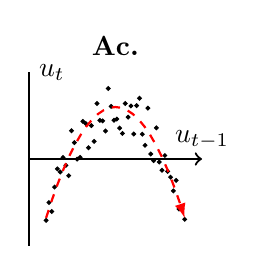
\begin{tikzpicture}[scale=0.11]
						% \draw [step=1, gray, very thin] (0, 0) grid (20, 23);
						\node at (10, 23) {\textbf{Ac.}}; 
						\draw [thick, ->] (0, 10) -- (20, 10) node [anchor=south] {$u_{t - 1}$}; 
						\draw [thick, -] (0, 0) -- (0, 20) node [anchor=west] {$u_{t}$}; 
						\draw plot [only marks, mark=*, mark size=6, domain=2:18, samples=50] (\x, {-0.2*(\x - 10)^2 + 13 + 6*rnd}); 
						\draw [thick, dashed, red, -latex] plot [domain=2:18] (\x, {-0.2*(\x - 10)^2 + 16});
					\end{tikzpicture}
				\end{center}
				
				\columnbreak
				
				\begin{center}
					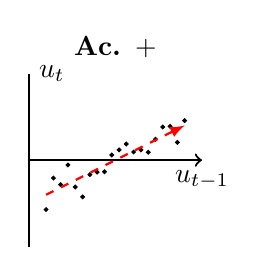
\begin{tikzpicture}[scale=0.11]
						% \draw [step=1, gray, very thin] (0, 0) grid (20, 23);
						\node at (10, 23) {\textbf{Ac. $+$}}; 
						\draw [thick, ->] (0, 10) -- (20, 10) node [anchor=north] {$u_{t - 1}$}; 
						\draw [thick, -] (0, 0) -- (0, 20) node [anchor=west] {$u_{t}$}; 
						\draw plot [only marks, mark=*, mark size=6, domain=2:18, samples=20] (\x, {5*rnd + 2.5 + 0.5*\x}); 
						\draw [thick, dashed, red, -latex] plot [domain=2:18] (\x, {5 + 0.5*\x});
					\end{tikzpicture}
				\end{center}
				
				\columnbreak
				
				\begin{center}
					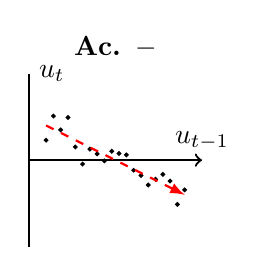
\begin{tikzpicture}[scale=0.11]
						% \draw [step=1, gray, very thin] (0, 0) grid (20, 23);
						\node at (10, 23) {\textbf{Ac. $-$}}; 
						\draw [thick, ->] (0, 10) -- (20, 10) node [anchor=south] {$u_{t - 1}$}; 
						\draw [thick, -] (0, 0) -- (0, 20) node [anchor=west] {$u_{t}$}; 
						\draw plot [only marks, mark=*, mark size=6, domain=2:18, samples=20] (\x, {5*rnd + 12.5 - 0.5*\x}); 
						\draw [thick, dashed, red, -latex] plot [domain=2:18] (\x, {15 - 0.5*\x});
					\end{tikzpicture}
				\end{center}
			\end{multicols}
			
			\begin{multicols}{2}
				\item \textbf{Correlograma} - compuesto de la función de autocorrelación (FAC) y el FAC parcial (FACP).
				
				\columnbreak
				
				\begin{itemize}[leftmargin=*]
					\item Eje Y: correlación [-1, 1].
					\item Eje X: número de retardo.
					\item Líneas azules: $\pm 1.96/T^{0.5}$
				\end{itemize}
			\end{multicols}
			
			\begin{center}
				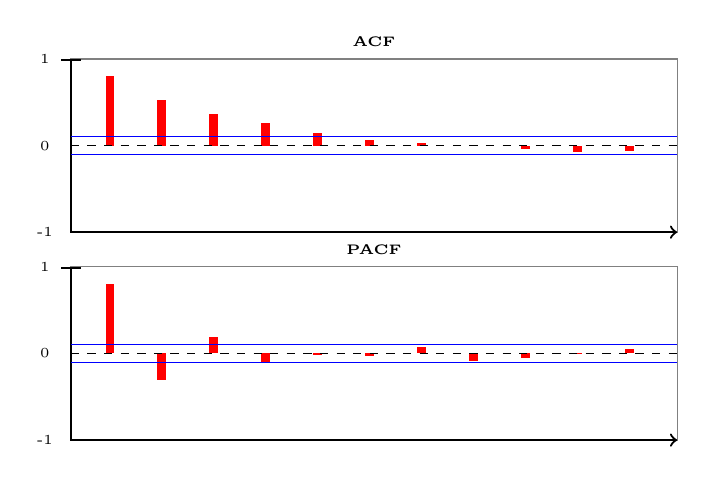
\begin{tikzpicture}[scale=0.22]
					% acf plot
					\node at (17.5, 23) {\tiny \textbf{ACF}}; 
					\node at (-1.5, 22) {\tiny 1};
					\node at (-1.5, 17) {\tiny 0}; 
					\node at (-1.5, 12) {\tiny -1}; 
					\draw [step=2, gray, thin] (0, 12) rectangle (35, 22); 
					\draw [thick, |->] (0, 22) -- (0, 12) -- (35, 12); 
					\fill [red] (2.0, 17) rectangle (2.5, 21.00);
					\fill [red] (5.0, 17) rectangle (5.5, 19.64); 
					\fill [red] (8.0, 17) rectangle (8.5, 18.85); 
					\fill [red] (11.0, 17) rectangle (11.5, 18.28);
					\fill [red] (14.0, 17) rectangle (14.5, 17.74);
					\fill [red] (17.0, 17) rectangle (17.5, 17.31);
					\fill [red] (20.0, 17) rectangle (20.5, 17.17);
					\fill [red] (23.0, 17) rectangle (23.5, 17.05);
					\fill [red] (26.0, 17) rectangle (26.5, 16.80);
					\fill [red] (29.0, 17) rectangle (29.5, 16.62);
					\fill [red] (32.0, 17) rectangle (32.5, 16.67);
					\draw [blue, thin] (0, 17.5) -- (35, 17.5); 
					\draw [dashed, thin] (0, 17) -- (35, 17); 
					\draw [blue, thin] (0, 16.5) -- (35, 16.5);
					% pacf plot
					\node at (17.5, 11) {\tiny \textbf{PACF}}; 
					\node at (-1.5, 10) {\tiny 1}; 
					\node at (-1.5, 5) {\tiny 0}; 
					\node at (-1.5, 0) {\tiny -1}; 
					\draw [step=2, gray, thin] (0, 0) rectangle (35, 10);
					\draw [thick, |->] (0, 10) -- (0, 0) -- (35, 0); 
					\fill [red] (2.0, 5) rectangle (2.5, 9.00);
					\fill [red] (5.0, 5) rectangle (5.5, 3.47);
					\fill [red]	(8.0, 5) rectangle (8.5, 5.94);
					\fill [red] (11.0, 5) rectangle (11.5, 4.43);
					\fill [red] (14.0, 5) rectangle (14.5, 4.89);
					\fill [red] (17.0, 5) rectangle (17.5, 4.86);
					\fill [red] (20.0, 5) rectangle (20.5, 5.38);
					\fill [red] (23.0, 5) rectangle (23.5, 4.56);
					\fill [red] (26.0, 5) rectangle (26.5, 4.76);
					\fill [red] (29.0, 5) rectangle (29.5, 5.01);
					\fill [red] (32.0, 5) rectangle (32.5, 5.24);
					\draw [blue, thin] (0, 5.5) -- (35, 5.5); 
					\draw [dashed, thin] (0, 5) -- (35, 5); 
					\draw [blue, thin] (0, 4.5) -- (35, 4.5);
				\end{tikzpicture}
			\end{center}
			
			Conclusiones difieren entre procesos de autocorrelación.
			
			\columnbreak
			
			\begin{itemize}[leftmargin=*]
				\item \textbf{Proceso MA($q$)}. \textbf{FAC}: sólo los $q$ primeros coeficientes son significativos, el resto se anulan bruscamente. \textbf{FACP}: decrecimiento rápido exponencial atenuado u ondas sinusoidales.
				\item \textbf{Proceso AR($p$)}. \textbf{FAC}: decrecimiento rápido exponencial atenuado u ondas sinusoidales. \textbf{FACP}: sólo los $p$ primeros coeficientes son significativos, el resto se anulan bruscamente.
				\item \textbf{Proceso ARMA($p, q$)}. \textbf{FAC} y \textbf{FACP}: los coeficientes no se anulan bruscamente y presentan un decrecimiento rápido.
			\end{itemize}
			
			Si los coeficientes de la FAC no decaen rápidamente, hay claro indicio de falta de estacionariedad en media, lo que llevaría a tomar primeras diferencias en la serie original.
			
			\item \textbf{Contrastes} - Generalmente, $H_{0}$: No autocorrelación.
			
			Suponiendo que $u_{t}$ sigue un proceso AR(1):
			
			\begin{center}
				$u_{t} = \rho_{1} u_{t - 1} + \varepsilon_{t}$
			\end{center}
			
			donde $\varepsilon_{t}$ es ruido blanco.
			
			\begin{itemize}[leftmargin=*]
				\item \textbf{Prueba t AR(1)} (regresores exógenos):
				
				\begin{center}
					$t = \frac{\hat{\rho}_{1}}{\se(\hat{\rho}_{1})} \sim t_{T - k - 1, \alpha/2}$
				\end{center}
				
				\begin{itemize}[leftmargin=*]
					\item $H_{1}$: Autocorrelación de orden uno, AR(1).
				\end{itemize}
				
				\item \textbf{Estadístico Durbin-Watson} (regresores exógenos y normalidad de residuos):
				
				\begin{center}
					$d = \frac{\sum_{t=2}^{n} (\hat{u}_{t} - \hat{u}_{t - 1})^{2}}{\sum_{t=1}^{n} \hat{u}_{t}^{2}} \approx 2 \cdot (1 - \hat{\rho}_{1}), \; 0 \leq d \leq 4$
				\end{center}
				
				\begin{itemize}[leftmargin=*]
					\item $H_{1}$: Autocorrelación de orden uno, AR(1).
				\end{itemize}
				
				\begin{center}
					\scalebox{0.8}{
						\begin{tabular}{| c | c | c | c |}
							\hline
							$d =$          & 0 & 2 & 4  \\ \hline
							$\rho \approx$ & 1 & 0 & -1 \\ \hline
						\end{tabular}
					}
					
					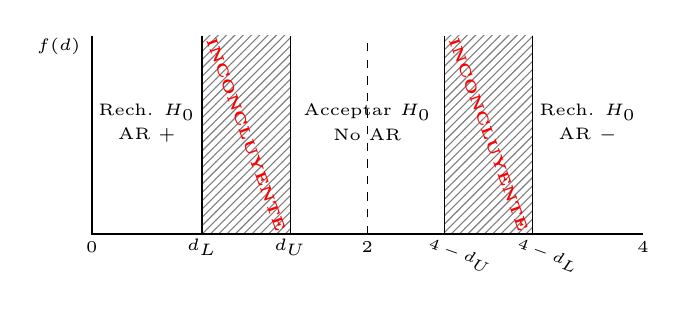
\begin{tikzpicture}[scale=0.28]
						\fill [pattern=north east lines, pattern color=gray] (5, 0) rectangle (9, 9); 
						\draw (5, 0) -- (5, 9); 
						\draw (9, 0) -- (9, 9); 
						\fill [pattern=north east lines, pattern color=gray] (16, 0) rectangle (20, 9); 
						\draw (16, 0) -- (16, 9); 
						\draw (20, 0) -- (20, 9); 
						\draw [thick] (0, 9) -- (0, 0) -- (25, 0); 
						\draw [dashed] (12.5, 0) -- (12.5, 9); 
						\node at (-1.5, 8.5) {\scalebox{1.2}{\tiny $f(d)$}}; 
						\node at (0, -0.6) {\scalebox{1.2}{\tiny 0}}; 
						\node at (5, -0.6) {\scalebox{1.2}{\tiny $d_{L}$}};
						\node at (9, -0.6) {\scalebox{1.2}{\tiny $d_{U}$}}; 
						\node at (12.5, -0.6) {\scalebox{1.2}{\tiny 2}}; 
						\node at (16.7, -1) {\scalebox{1.1}{\tiny \rotatebox{-20}{$4 - d_{U}$}}}; 
						\node at (20.7, -1) {\scalebox{1.1}{\tiny \rotatebox{-20}{$4 - d_{L}$}}}; 
						\node at (25, -0.6) {\scalebox{1.2}{\tiny 4}}; 
						\node at (2.5, 5.5) {\scalebox{1.2}{\tiny Rech. $H_{0}$}}; 
						\node at (2.5, 4.5) {\scalebox{1.2}{\tiny AR $+$}}; 
						\node [text=red] at (7, 4.5) {\scalebox{1.1}{\tiny \rotatebox{-70}{\textbf{INCONCLUYENTE}}}}; 
						\node at (12.5, 5.5) {\scalebox{1.2}{\tiny Acceptar $H_{0}$}}; 
						\node at (12.5, 4.5) {\scalebox{1.2}{\tiny No AR}}; 
						\node [text=red] at (18, 4.5) {\scalebox{1.1}{\tiny \rotatebox{-70}{\textbf{INCONCLUYENTE}}}}; 
						\node at (22.5, 5.5) {\scalebox{1.2}{\tiny Rech. $H_{0}$}}; 
						\node at (22.5, 4.5) {\scalebox{1.2}{\tiny AR $-$}};
					\end{tikzpicture}
				\end{center}
				
				\item \textbf{h de Durbin} (regresores endógenos):
				
				\begin{center}
					$h = \hat{\rho} \cdot \sqrt{\frac{T}{1 - T \cdot \upsilon}}$
				\end{center}
				
				donde $\upsilon$ es la varianza estimada del coeficiente asociado a la variable endógena.
				
				\begin{itemize}[leftmargin=*]
					\item $H_{1}$: Autocorrelación de orden uno, AR(1).
				\end{itemize}
				
				\item \textbf{Prueba Breusch-Godfrey} (regresores endógenos): puede detectar procesos MA($q$) y AR($p$) ($\varepsilon_{t}$ ruido b.):
				
				\begin{itemize}[leftmargin=*]
					\item MA($q$): $u_{t} = \varepsilon_{t} - m_{1} u_{t - 1} - \cdots - m_{q} u_{t - q}$
					\item AR($p$): $u_{t} = \rho_{1} u_{t - 1} + \cdots + \rho_{p} u_{t - p}+ \varepsilon_{t}$
				\end{itemize}
				
			\columnbreak
				
				Bajo $H_{0}$: No autocorrelación:
				
				\begin{center}
					$\hfill T \cdot R^{2}_{\hat{u}_t}\underset{a}{\sim}\chi^{2}_{q} \hfill \textbf{or} \hfill T \cdot R^{2}_{\hat{u}_t}\underset{a}{\sim}\chi^{2}_{p} \hfill$
				\end{center}
				
				\begin{itemize}[leftmargin=*]
					\item $H_{1}$: Autocorrelación de orden $q$ (ó $p$).
				\end{itemize}
				
				\item \textbf{Prueba Ljung-Box Q}:
				
				\begin{itemize}[leftmargin=*]
					\item $H_{1}$: Existe autocorrelación.
				\end{itemize}
			\end{itemize}
		\end{itemize}
		
		\subsection*{Corrección}
		
		\begin{itemize}[leftmargin=*]
			\item Usar MCO con un estimador de la matriz de varianzas-covarianzas \textbf{robusto a la heterocedasticidad y autocorrelación} (HAC), por ejemplo, la propuesta de \textbf{Newey-West}.
			\item Usar \textbf{Mínimos Cuadrados Generalizados} (MCG). Suponiendo $y_{t} = \beta_{0} + \beta_{1} x_{t} + u_{t}$, con $u_{t} = \rho u_{t - 1}+ \varepsilon_{t}$, donde $\lvert \rho \rvert < 1$ y $\varepsilon_{t}$ es \underline{ruido blanco}.
			
			\begin{itemize}[leftmargin=*]
				\item Si $\rho$ es \textbf{conocido}, usar \textbf{modelo cuasi-diferenciado}:
			
				\begin{center}
					$y_{t} - \rho y_{t - 1}= \beta_{0} (1 - \rho) + \beta_{1} (x_{t} - \rho x_{t - 1}) + u_{t} - \rho u_{t - 1}$
					
					$y_{t}^{*} = \beta_{0}^{*} + \beta_{1}' x_{t}^{*} + \varepsilon_{t}$
				\end{center}
				
				donde $\beta_{1}' = \beta_{1}$; y estimarlo por MCO.
				
				\item Si $\rho$ es \textbf{desconocido}, estimarlo -por ejemplo- el \textbf{método iterativo de Cochrane-Orcutt} (el método de Prais-Winsten también es bueno):
				
				\begin{enumerate}[leftmargin=*]
					\item Obtener $\hat{u}_{t}$ del modelo original.
					\item Estimar $\hat{u}_{t} = \rho \hat{u}_{t-1} + \varepsilon_{t}$ y obtener $\hat{\rho}$.
					\item Crear un modelo cuasi-diferenciado:
					
					\begin{center}
						$y_{t} - \hat{\rho}y_{t - 1} = \beta_{0} (1 - \hat{\rho}) + \beta_{1} (x_{t} - \hat{\rho} x_{t - 1}) + u_{t} - \hat{\rho}u_{t - 1}$
						
						$y_{t}^{*} = \beta_{0}^{*} + \beta_{1}' x_{t}^{*} + \varepsilon_{t}$
					\end{center}
					
					donde $\beta_{1}' = \beta_{1}$; y estimarlo por MCO.
					
					\item Obtener $\hat{u}_{t}^{*} = y_{t} - (\hat{\beta}_{0}^{*} + \hat{\beta}_{1}' x_{t}) \neq y_{t} - (\hat{\beta}_{0}^{*} + \hat{\beta}_{1}' x_{t}^{*})$.
					\item Repetir desde el paso 2. El algoritmo termina cuando los parámetros estimados varían muy poco entre iteraciones.
				\end{enumerate}
			\end{itemize}
			
			\item Si no se arregla, buscar \textbf{fuerte dependencia} en la serie.
		\end{itemize}
		
		\section*{Suavizado exponencial}
		
		\begin{center}
			$f_{t} = \alpha y_{t} + (1 - \alpha) f_{t - 1}$
		\end{center}
		
		donde $0 < \alpha < 1$ es el parámetro de suavizado.
		
		\section*{Predicciones}
		
		Dos tipos de predicciones:
		
		\begin{itemize}[leftmargin=*]
			\item Valor medio de $y$ para un valor específico de $x$.
			\item Valor individual de $y$ para un valor específico de $x$.
		\end{itemize}
		
		\columnbreak
		
		\section*{Estacionariedad}
		
		La estacionariedad permite reconocer relaciones --inalteradas en el tiempo-- entre variables.
		
		\begin{itemize}[leftmargin=*]
			\item \textbf{Proceso estacionario} (estacionariedad estricta) - si se toma cualquier colección de variables aleatorias y se mueven $h$ periodos (el tiempo cambia), la distribución conjunta de probabilidades debe permanecer inalterada.
			\item \textbf{Proceso no estacionario} - por ejemplo, una serie con tendencia, donde al menos la media cambia con el tiempo.
			\item \textbf{Proceso estacionario en covarianza} - es una forma más débil de estacionariedad:
			
			\begin{itemize}[leftmargin=*]
				\begin{multicols}{2}
					\item $\E(x_{t})$ es constante.
					
					\columnbreak
					
					\item $\Var(x_{t})$ es constante.
				\end{multicols}
				
				\item Para cualquier $t$, $h \geq 1$, la $\Cov(x_{t}, x_{t + h})$ depende sólo de $h$, no de $t$.
			\end{itemize}
		\end{itemize}
		
		\section*{Dependencia débil}
		
		La dependencia débil reemplaza el supuesto de muestreo aleatorio en series temporales.
		
		\begin{itemize}[leftmargin=*]
			\item Un proceso estacionario $\lbrace x_{t} \rbrace$ es \textbf{débilmente dependiente} cuando $x_{t}$ y $x_{t + h}$ son casi independientes a medida que $h$ aumenta sin límite.
			\item Un proceso estacionario en covarianza es \textbf{débilmente dependiente} si la correlación entre $x_{t}$ y $x_{t + h}$ tiende a $0$ lo suficientemente rápido cuando $h \rightarrow \infty$ (no están asintóticamente correlacionados).
		\end{itemize}
		
		Los procesos débilmente dependientes se llaman \textbf{integrados de orden cero}, I(0). Algunos ejemplos:
		
		\begin{itemize}[leftmargin=*]
			\item \textbf{Media móvil} - $\lbrace x_{t} \rbrace$ es una media móvil de orden $q$, MA($q$):
			
			\begin{center}
				$x_{t} = e_{t} + m_{1} e_{t - 1} + \cdots + m_{q} e_{t - q}$
			\end{center}
			
			donde $\lbrace e_{t} : t = 0, 1, \ldots, T \rbrace$ es una secuencia \textsl{i.i.d.} con media cero y varianza $\sigma^{2}_{e}$.
			
			\item \textbf{Proceso autorregresivo} - $\lbrace x_{t} \rbrace$ es un proceso autorregresivo de orden $p$, AR($p$):
			
			\begin{center}
				$x_{t} = \rho_{1} x_{t - 1} + \cdots + \rho_{p} x_{t - p} + e_{t}$
			\end{center}
			
			donde $\lbrace e_{t}: t = 1, 2, \ldots, T \rbrace$ es una secuencia \textsl{i.i.d.} con media cero y varianza $\sigma^{2}_{e}$.
			
			\textbf{Condición de estabilidad}: si $1 - \rho_{1} z - \cdots - \rho_{p} z^{p} = 0$ para $\lvert z \rvert > 1$, entonces $\lbrace x_{t} \rbrace$ es un proceso AR débilmente dependiente. Para AR(1), la condición es: $\lvert \rho_{1} \rvert < 1$.
		
			\item \textbf{Proceso ARMA} - es una combinación de los dos anteriores; $\lbrace x_{t} \rbrace$ es un ARMA($p, q$):
			
			\begin{center}
				$x_{t} = e_{t} + m_{1} e_{t - 1} + \cdots + m_{q} e_{t - q} + \rho_{1} x_{t - 1} + \cdots + \rho_{p} x_{t - p}$
			\end{center}
		\end{itemize}
		
		\columnbreak
		
		\section*{Raíces unitarias}
		
		Un proceso es I($d$), esto es, integrado de orden $d$, si al aplicar diferencias $d$ veces hace al proceso estacionario.
		
		Cuando $d \geq 1$, al proceso se le llama \textbf{proceso de raíz unitaria} o se dice que tiene una raíz unitaria.
		
		Un proceso tiene una raíz unitaria cuando la condición de estabilidad no se cumple (hay raíces en el círculo unitario).
		
		\subsection*{Dependencia fuerte}
		
		La mayoría del tiempo, las series económicas presentan dependencia fuerte (o fuerte persistencia temporal). Algunos casos especiales de procesos de \textbf{raíz unitaria} I(1):
		
		\begin{itemize}[leftmargin=*]
			\item \textbf{Paseo aleatorio} - un proceso AR(1) con $\rho_{1} = 1$.
			
			\begin{center}
				$y_{t} = y_{t - 1} + e_{t}$
			\end{center}
			
			donde $\lbrace e_{t} : t = 1, 2, \ldots, T \rbrace$ es una secuencia \textsl{i.i.d.} con media cero y varianza $\sigma^{2}_{e}$.
			
			\item \textbf{Paseo aleatorio con deriva} - un proceso AR(1) con $\rho_{1} = 1$ y una constante.
			
			\begin{center}
				$y_{t} = \beta_{0} + y_{t - 1} + e_{t}$
			\end{center}
			
			donde $\lbrace e_{t} : t = 1, 2, \ldots, T \rbrace$ es una secuencia \textsl{i.i.d.} con media cero y varianza $\sigma^{2}_{e}$.
		\end{itemize}
		
		\subsection*{Contrastes de raíz unitaria}
		
		\begin{center}
			\begin{tabular}{ c | c | c }
				Contraste       & $H_{0}$        & Rechazar $H_{0}$                  \\ \hline
				ADF             & I(1)           & tau \textless \, Valor crítico    \\ \hline
				KPSS            & I(0) nivel     & mu \textgreater \, Valor crítico  \\
				                & I(0) tendencia & tau \textgreater \, Valor crítico \\ \hline
				Phillips-Perron & I(1)           & Z-tau \textless \, Val. crítico   \\ \hline
				Zivot-Andrews   & I(1)           & tau \textless \, Valor crítico
			\end{tabular}
		\end{center}
		
		\subsection*{De raíz unitaria a dependencia débil}
		
		Integrado de \textbf{orden uno}, I(1), significa que \textbf{la primera diferencia} del proceso es \textbf{débilmente dependiente} ó I(0) (y usualmente, estacionaria). Por ejemplo, sea $\lbrace y_{t} \rbrace$ un paseo aleatorio:
		
		\begin{multicols}{2}
			\begin{center}
				$\Delta y_{t} = y_{t} - y_{t - 1} = e_{t}$
			\end{center}
			
			donde $\lbrace e_{t} \rbrace = \lbrace \Delta y_{t} \rbrace$ es \textsl{i.i.d.} \\

			Nota:
			\begin{itemize}[leftmargin=*]
				\item La primera diferencia de una serie elimina su tendencia.
				\item El logaritmo de una serie estabiliza su varianza.
			\end{itemize}
			
			\columnbreak
			
			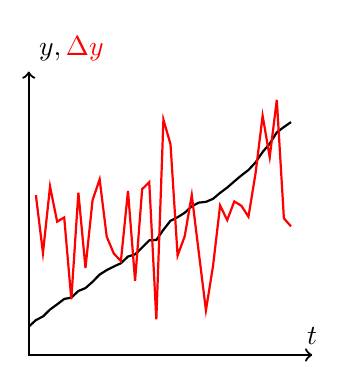
\begin{tikzpicture}[scale=0.18]
				% \draw [step=1, gray, very thin] (0, 0) grid (20, 20); 
				\draw [thick, <->] (0, 20) node [anchor=south west] {$y, {\color{red} \Delta y}$} -- (0, 0) -- (20, 0) node [anchor=south] {$t$}; 
				\draw [thick, black] 
				(0.0, 2.000) -- (0.5, 2.459) -- 
				(1.0, 2.716) -- (1.5, 3.205) -- 
				(2.0, 3.571) -- (2.5, 3.952) -- 
				(3.0, 4.047) -- (3.5, 4.514) -- 
				(4.0, 4.719) -- (4.5, 5.160) -- 
				(5.0, 5.674) -- (5.5, 5.987) -- 
				(6.0, 6.242) -- (6.5, 6.471) -- 
				(7.0, 6.944) -- (7.5, 7.104) -- 
				(8.0, 7.584) -- (8.5, 8.087) -- 
				(9.0, 8.112) -- (9.5, 8.834) -- 
				(10.0, 9.470) -- (10.5, 9.718) -- 
				(11.0, 10.032) -- (11.5, 10.491) -- 
				(12.0, 10.748) -- (12.5, 10.805) -- 
				(13.0, 11.016) -- (13.5, 11.439) --
				(14.0, 11.810) -- (14.5, 12.247) -- 
				(15.0, 12.668) -- (15.5, 13.052) -- 
				(16.0, 13.586) -- (16.5, 14.322) -- 
				(17.0, 14.913) -- (17.5, 15.704) -- 
				(18.0, 16.081) -- (18.5, 16.431); 
				\draw [thick, red] 
				(0.5, 11.283) -- (1.0, 7.201) -- 
				(1.5, 11.889) -- (2.0, 9.405) -- 
				(2.5, 9.701) -- (3.0, 3.926) -- 
				(3.5, 11.454) -- (4.0, 6.136) -- 
				(4.5, 10.926) -- (5.0, 12.393) -- 
				(5.5, 8.345) -- (6.0, 7.157) -- 
				(6.5, 6.627) -- (7.0, 11.572) -- 
				(7.5, 5.235) -- (8.0, 11.703) -- 
				(8.5, 12.186) -- (9.0, 2.513) -- 
				(9.5, 16.607) -- (10.0, 14.869) -- 
				(10.5, 7.015) -- (11.0, 8.368) -- 
				(11.5, 11.283) -- (12.0, 7.196) -- 
				(12.5, 3.153) -- (13.0, 6.277) -- 
				(13.5, 10.547) -- (14.0, 9.517) -- 
				(14.5, 10.834) -- (15.0, 10.526) -- 
				(15.5, 9.754) -- (16.0, 12.816) -- 
				(16.5, 16.875) -- (17.0, 13.961) -- 
				(17.5, 18.000) -- (18.0, 9.644) -- 
				(18.5, 9.075);
			\end{tikzpicture}
		\end{multicols}
		
		\columnbreak
		
		\subsubsection*{De raíz unitaria a cambio porcentual}
		
		Cuando una serie I(1) es estrictamente positiva, se suele transformar a logaritmos antes de tomar primeras diferencias para obtener el cambio porcentual (aprox.) de la serie:
		
		\begin{center}
			$\Delta \log(y_{t}) = \log(y_{t}) - \log(y_{t - 1}) \approx \dfrac{y_t - y_{t - 1}} {y_{t - 1}}$
		\end{center}
		
		\section*{Cointegración}
		
		Cuando \textbf{dos series son I(1), pero una combinación lineal de estas es I(0)}. Si es el caso, la regresión de una serie sobre la otra no es espuria, sino que expresa algo sobre la relación a largo plazo. Se llama cointegradas a las variables que tienen una tendencia estocástica común.
		
		Por ejemplo, $\lbrace x_{t} \rbrace$ y $\lbrace y_{t} \rbrace$ son I(1), pero $y_{t} - \beta x_{t} = u_{t}$ donde $\lbrace u_{t} \rbrace$ es I(0). ($\beta$ es el parámetro cointegrador).
		
		\subsection*{Contraste de cointegración}

		Siguiendo el ejemplo de arriba:
		
		\begin{enumerate}[leftmargin=*]
			\item Estimar $y_{t} = \alpha + \beta x_{t} + \varepsilon_{t}$ y obtener $\hat{\varepsilon}_{t}$
			\item Realizar el ADF sobre $\hat{\varepsilon}_{t}$ con una distribución especial.
			
			El resultado del contraste es equivalente a:
			
			\begin{itemize}[leftmargin=*]
				\item $H_{0}$: $\beta = 0$ (no cointegración)
				\item $H_{1}$: $\beta \neq 0$ (cointegración)
			\end{itemize}
			
			si el estadístico de contraste $>$ valor crítico, rechazar $H_0$.
		\end{enumerate}

		\section*{Heterocedasticidad en series temp.}
		
		Afecta al \textbf{supuesto t4}, lo que lleva a que \textbf{MCO no sea eficiente}.
		
		Usar contrastes como el Breusch-Pagan o White, donde $H_{0}$: No heterocedasticidad. Es \textbf{importante} que \textbf{no} haya \textbf{autocorrelación} para que los contrastes funcionen.
		
		\subsection*{ARCH}
		
		Heterocedasticidad condicional autorregresiva (ARCH), es un modelo para analizar una forma de heteroced. dinámica, donde la varianza del error sigue un proceso AR($p$).
		
		Dado el modelo: $y_{t} = \beta_{0} + \beta_{1} z_{t} + u_{t}$ donde, hay AR(1) y heterocedasticidad:
		
		\begin{center}
			$\E(u^{2}_{t} \mid u_{t - 1}) = \alpha_{0} + \alpha_{1} u^{2}_{t - 1}$
		\end{center}
		
		\subsection*{GARCH}
		
		Heterocedasticidad condicional autorregresiva general (GARCH), es un modelo similar a ARCH, pero en este caso, la varianza del error sigue un proceso ARMA($p, q$).
	\end{multicols}
\end{document}